% 2.1
\section{Den aggregatorienterte datamodellen}

% Først, introduser og definer begrepet ''aggregatorientert datamodell'' - Kanskje jeg bør forklare ytterligere hva det betyr?
Ifølge \cite{sadalage2013} kan nøkkel-verdi-lagre (eng. key-value store), kolonnefamilielagre (eng. column family stores) og dokumentlagre (eng. ''document stores'') ordnes under én og samme ''art'' av NoSQL-databaser: Aggregatorienterte databasesystem (eng. ''aggregate oriented databases''). Denne introduksjonen til de tre nevnte NoSQL - datamodellene forholder seg til denne klassifiseringen. Utover disse tre typene av NoSQL - modeller finnes også den graforienterte modellen, som benyttes av systemer som InfiniteGraph, OrientDB og FlockDB. Denne datamodellen vil ikke bli beskrevet i noen videre detalj.

Dette delkapitlet begynner med å beskrive den relasjonelle datamodellen, og hvorfor den ikke holder mål i et distribuert produksjonsmiljø der større datavolum behandles. Dernest blir den aggregatorienterte datamodellen beskrevet, en kategori av NoSQL-modeller som denoterer fellesnevneren mellom nøkkel-verdi-lagre, dokumentlagre og kolonnefamilielagre. Samtlige tre former for aggregatorientering beskrives i avsnitt 3 til 5.

% Hovedkjelder: sadalage2013 + pensum fra egne fag
% Før første subseksjon: Om relasjonelle modeller, motivasjonen bak NoSQL; 2.1.3: Nøkkel-verdi-lagre; 2.1.4: Dokumentlagre; 2.1.5: KFL; 2.1.2 Ett eget overordnet kapittel om aggregatorientering; 2.1.1 mySQL?

% 2.1.1
\subsection{Den relasjonelle datamodellen}

% Den relasjonelle datamodellen, i.e. MariaDB og Postgres (Bøyningen av sybstantivet 'tuppel' samsvarer med Bratsbergengens skrivemåte i hans artikkel om relasjonsdatabaser hos SNL)
Den enkleste måten å forklare hva den aggregatorienterte datamodellen er, er ved først å beskrive hva den ikke er. I den relasjonelle datamodellen organiseres forskjellige former for applikasjonsdata inn i relasjoner, og data tilhørende samme relasjon inndeles i atomiske, disjunkte enheter kalt \emph{tupler}. En tuppel er en flat, endimensjonal liste av dataverdier. Hver av disse verdiene korresponderer til nøyaktig ett attributt av relasjonen tuppelen er lagret i.

% Strukturelle begrensninger i relasjonsdatabaser
Det foreligger visse begrensninger på denne datastrukturen. Til eksempel kan ikke en enkelt tuppel nøstes inn i en annen, og hvert attributt i tuppelen har én atomisk korresponderende verdi, aldri en liste av verdier. Nå skal det sies at nyere versjoner av MariaDB støtter JSON-objekter som datatype \citep{mariadb}. JSON-objekter er serialiserte (dsv konverterte til strenger), fleksible dataenheter som kan inneholde nøstede datastrukturer.

Imidlertid har ikke databasesystemet noen forståelse for de enkelte dataelementer som objektet innkapsler, det ser bare en helhetlig, ugjennomsiktlig dataenhet, nemlig verdien av ett attributt i relasjonen. Ettersom tupler er den minste, udelelige dataenheten i den relasjonelle modellen er det korrekt å fastslå at spørringer opererer med og returnerer (et helt antall) tupler for hver enkelt spørring \citep{sadalage2013}. Riktignok går det an å utvelge distinkte attributter i spørringen, også kjent som kommandoen \texttt{PROJECT} i relasjonell algebra, likefullt er den tellbare dataenheten i resultantrelasjonen tupler, også referert til som rader i kontekst av databaseapplikasjoner.

% Spørringsfleksibilitet (JOIN + avanserte operasjoner) - Fra databasepensum
Følgelig gir slike strengt strukturerte datamodeller stor fleksibilitet for spørringene som utføres av databasesystemet. Det kan for eksempel samle sammen alle verdier for ett spesifikt numerisk attributt i én bestemt relasjon, summere disse  attributtverdiene sammen og returnere resultatet som et separat attributt i resultanttuppelen. På samme vis kan relasjonsdatabasesystemet kalkulere gjennomsnittet for alle eller enkelte av tuplene i en relasjon, telle opp antallet tupler i den, finne den høyeste numeriske verdien eller finne den laveste.

Ved hjelp av JOIN-operasjoner finner man eksisterende tupler fra forskjellige relasjoner, relatert til hverandre via fremmednøkler, og resultanten av JOINen kan systemet også kalle disse aggregeringsoperasjonene på. NoSQL - databaser har ikke den samme fleksibiliteten til selv å utføre slike spørreoperasjoner: Hver spørring henter kun én dataenhet ad gangen, noe som holder især for nøkkelverdilagre. Hver spørring er logisk sett bare et oppslag på en nøkkel i en hashtabell. Eventuell aggregering der sum, gjennomsnitt eller ekstremalverdier regnes må gjøres i selve applikasjonen, etter at oppslag på \textbf{samtlige} nøkler er gjort i databasen.

% Figur 1
\begin{figure}[h]
    \centering
    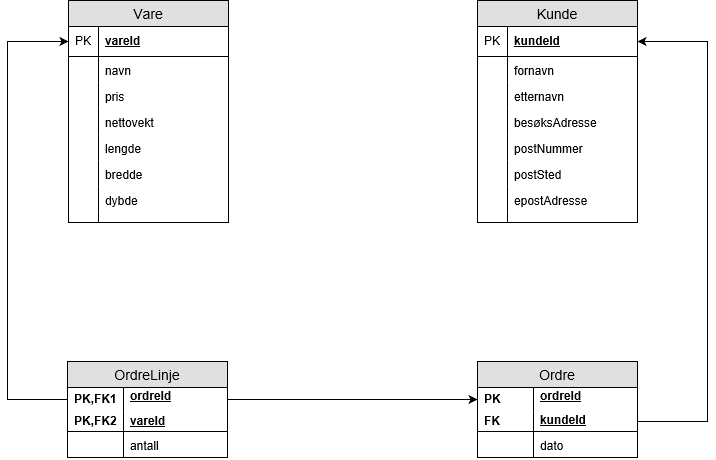
\includegraphics{fig/NettbutikkOrdreModell}
    \caption{Diagram over tabeller i en relasjonsdatabase som registrerer ordrer fra kunder i en netthandelapplikasjon.}
    \label{fig1}
\end{figure}
 
% Impedansproblemet (Impedance mismatch problem)
I en typisk netthandelapplikasjon er applikasjonens datamodell denotert i form av dataobjekter midlertidig lagret i primærminnet, mer presist sagt, i adresseområdet til èn, eller flere, av nettleserens kjørende prosesser i kundens datamaskin. Variablene i datafeltene i disse objektene kan være saå mangt: strenger, tall, referenser til andre objekter, lister bestående av ovennevnte typer.. Disse dataobjektene endres i sanntid av kunden som aksesserer nettbutikken gjennom standardiserte interaksjonselementer som tekstfelt, knapper, slidere, sjekkbokser og radiobokser, gruppert sammen i dynamiske sideelementer kjent som skjema (eng. ''form''). Et praktisk eksempel på et skjema i en netthandel er handlevognen, som viser kunden hvilke vareartikler han (foreløpig) vil kjøpe, hvor mange av hver vare som ''ligger'' i handlevogna, og hvor mye varene koster sammenlagt.

Når det kommer til å skrive dataene fra web-skjemaet til disk i en relasjonsdatabase ser ting annerledes ut. Her persisteres data om varer (navn, identifikasjonsnummer størrelsesdimensjoner, nettovekt, og enhetspris \footnote{Gitt at hver enkelt vare-tuppel representerer en diskret enhet, til eksempel én bøtte maling eller én sekk med poteter}) til en egen relasjon. En annen relasjon holder data om kunder, en tredje holder på informasjon om bestillinger, og for normaliseringens skyld eksisterer en egen jointabell kalt Ordrelinje som kopler sammen Ordre og Vare, som illustrert i tabell-diagrammet i \ref{fig1}. Denne uoverensstemmelsen mellom strukteren av applikasjonsdata i programminne og strukturen på de samme dataene i en relasjonsdatabase refereres til i industrien som ''the impedance mismatch'' \citep{sadalage2013}.

Følgelig må applikasjonsutviklere konvertere data fra spørringsresultater til den dataobjektstrukturen applikasjonen påkrever, noe som per idag ofte løses ved å innføre et seperat abstrahert lag i applikasjonens logiske arkitektur: En tredjepartsmodul kalt ''object-relational mapper'' (ORM). For språket Java kan man bruke Hibernate\footnote{\url{http://hibernate.org/orm/}}, JavaScript har SequelizeJS\footnote{\url{http://docs.sequelizejs.com/}}, og PHP-utviklere kan bruke Doctrine\footnote{\url{http://www.doctrine-project.org/}}, som også er en del av webapplikasjonsrammeverket Symfony\footnote{\url{http://symfony.com/}}. Med slike tredjepartsbibliotek følger selvfølgelig et nytt mønster som utviklere blir nødt til å forholde seg skal de ta det i bruk. Ettersom det relasjonelle datalaget abstraheres bort er det tilforlatelig å ''glemme'' at applikasjonsdata faktisk persisteres i en relasjonell database. En tilsynelatende enkel henteoperasjon på objektform kan fort translatere til to kostbare JOIN-operasjoner i databasen som kjøres hver gang spørringen utføres.

% Distribuering av data utover flere instanser == katastrofe
En annen innvending mot den relasjonelle datamodellen involverer hvordan den støtter skalering av arbeidslast med hensyn på økende antall brukere, økende antall datakilder, økende antall . Datamodellen ble etablert på 70-tallet, i en æra lenge før datamaskinen ble allemanseie, et markedsskifte ingen av datidens eksperter kunne forutse. Relasjonsdatabaser er designet med tanke på monolittiske systemarkitekturer, programvarearkitekturer hvis system kjører på én enkel datamaskin, fordelt på et sett med prosesser innad i den. For et begrenset antall datakilder/brukere er slike systemer i noen grad vertikalt skalerbare, det vil si at økt last på systemet kan løses ved å oppgradere maskinvaren. Denne metoden er innlysende nok kostbar i det lange løp ettersom maskinvare som skiftes ut ikke er brukelig for systemet lengre. Da er det billigere å skalere horisontalt, det vil si å kjøre programvaresystemet i en klynge av datamaskiner sammenkoplet over et IP - nettverk. Som demonstrert i følgende eksempel statuert av \cite{george2011} skal vi se at å operere i klynget system ikke er så lett når data modelleres relasjonelt.

% Jamfør HBase - penusm i TDT4150
Hush er en (fiktiv) url-forkortelsestjeneste som i begynnelsen har omtrent et par tusen brukere, og vedlikeholdes og bygges med gratis tredjepartsmoduler, blant annet driftes en LAMP-tjener (Linux, Apache, MariaDB, PHP) som leverer en prototype av denne tjenesten i form av en webapplikasjon. Hush sin relasjonelle databasemodell normaliserer sine data ved å definere fire tabeller, \texttt{user}, \texttt{url}, \texttt{shorturl}, og \texttt{click} \citep{george2011}. De tre sistnevnte tabellene er assosiert med \texttt{user} gjennom en fremmednøkkel som refererer til nøkkelattributtet til den tabellen. I tillegg er brukertabellen og kort-URL-tabellen indeksert etter sine respektive nøkkelattributter for å gjøre oppslag på korte URLer og brukere raskere. Med transaksjoner sikrer man at de relaterte tabellene (den for URLer, korte URLer og klikk) endres sekvensielt og fullstendig slik at et strengt konsistensnivå opprettholdes tuplene imellom.

Denne monolittiske databasearkitekturen fungerer med det gitte antall brukere. Idet tjenesten blir verdenskjent, og antallet brukere øker eksponensielt med fire tierpotenser, blir arbeidslasten for databasetjeneren etter hvert for stor å handtere alene. Den naturlige løsningen på å tekkes vekstraten i databasens arbeidslast er å innføre flere databasetjenere installert på separate datamaskiner. Når skriveoperajsoner og leseoperajsoner i et databasesystem distribueres utover en klynge tjenere, er det viktig å organisere dem slik at arbeidslasten jevnfordeles metodisk slik at databasesystemets distribuerte natur ikke er synlig for applikasjonen som utfører spørringen. 

% 2.1.2
\subsection{Fellesnevneren for nøkkelverdilagre, kolonnefamilielagre, og dokumentlagre}

Så har vi den aggregatorienterte modellen, en måte å tenke på data som tillater den enkelte datamodellør å definere dataenheter i stedet for å tvinge vedkommende til å konformere med en forhåndsbestemt minste enhet, slik tilfellet er i den relasjonelle modellen. Denne fleksibiliteten i struktureringen av data er et sentralt fellestrekk nøkkel-verdi-lagre som Dynamo og Redis deler med kolonnefamilie-lagre som Cassandra og HBase og dokumentdatabaser som MongoDB og CouchDB. Derfor definerer \cite{sadalage2013} en felles kategori for disse tre NoSQL-typene: ''Aggregatorienterte databasesystem''.

Begrepet ''aggregat'' (må ikke forveksles med det matematiske verbet som betegner en operasjon på en gruppe av tupler) er lånt fra domenedrevet design og er definert som en samling sammenknyttede objekter som en datamodellør ønsker å behandle som en datamanipulasjonsenhet. Når komplekse aggregater aksesseres, gjøres det med et oppslag på én enkelt nøkkel, så får man både dataobjektet med den tilhørende nøkkelen samt eventuelle assosierte dataobjekter. Å utføre en tilsvarende lesing av to assosierte relasjoner i for eksempel MariaDB krever først oppslag i en tabell på dens nøkkelverdi, deretter enda et oppslag på en fremmednøkkel i den assosierte tabellen, altså må en JOIN-operasjon utføres.

Lesing av aggregerte dataobjekter medfører altså at man med ett enkelt oppslag får både i pose og sekk. Aggregatmodellen er også en enklere datamodell å forholde seg til for de som programmerer selve applikasjonen som behandler dataene. De enkelte aggregater, det vil si applikasjonsprogrammererens definisjon for databehandlingsenhet utgjør en naturlig enhet for replikering i en klynge av enkeltstående databasenoder. I et distribuert databasesystem gjelder det å minimalisere antall noder som kontaktes for hver spørring. Når konsepter settes sammen eksplisitt i datamodellen slik som vi ser i de fleksible dokumentstrukturene til Mongo, vet databasen hvilke dataenheter som skal aksesseres samtidig, og som derfor naturlig nok bør plasseres på én og samme node.

\cite{sadalage2013} kaller relasjonelle database og grafdatabaser for \textbf{aggregat-uvitende}. Deres datamodeller betrakter ikke aggregater eller sammensatte datastrukturer i deres dataoperasjoner. Aggregat-uvitenhet er ikke nødvendigvis et dårlig designvalg, ettersom det ikke alltid er opplagt for den enkelte webapplikasjonsutvikler hvilke enhetsbegrensinger i datamodellen som er logiske, iallfall ikke før datamodellen er definert for første gang og revidert to til tre ganger i løpet av utviklingsprosessen. Den lagrede dataen kan ha mange forskjellige brukskontekster, avhengig av applikasjonens funksjonelle krav som ofte blir forandret underveis i applikasjonens livssyklus.

En enkelt aggregatstruktur kan ikke medføre optimale spørringsytelse for alle mulige brukskontekster. Her gjelder det for utvikleren å prioritere den mest typiske leseoperasjonen tjenesten utsettes for. Hvis applikasjonen ikke har en slik primær aksess – struktur på dataobjektene kan man like godt modellere dem på et aggregat-uvitende vis. I en aggregat-uvitende modell har brukskonteksten ingen innvirkning på spørringen, fordi operasjonsenheten er én enkelt tuppel i MariaDB (én enkelt data-node i en grafdatabase som Orient) uansett hvordan konseptene er satt sammen.

Transaksjoner er en velprøvd og høyt akseptert logisk modell for databehandling. Relasjonelle databaser tillater oppdatering av eller lesing av tupler i opptil flere relasjoner innen et sett med atomiske operasjoner. Det er den enkelte mengden av hendelser som heter for en transaksjon. En transaksjon avgrenser mengden av hendelser og skriver enten samtlige eller ingen endringer til disk.

Transaksjonenes egenskaper beskrives med akronymet ACID: De er atomiske, dvs at samtlige hendelser i transaksjonen blir enten gjennomført fullstendig eller ei; konsistente (eng. ''Consistent''), dvs at to transaksjoner som kjører parallellt alltid medfører det samme sluttresultatet; isolerte, det vil si holdbare i den grad transaksjonen persisteres til disk (eng. ''Durable''). Transaksjonsmodellen fremmer en spesifikk handling, \texttt{COMMIT}, som signaliserer at endringene spesifisert i den enkelte transaksjon er blitt gjort permanente.

Aggregatorienterte databasesystemer innehar ikke ACID - egenskapene på samme vis som relasjonelle databasesystemer. Imidlertid støtter de naturlig atomiske manipulasjoner på ett eneste aggregat av gangen. Operasjoner på flere aggregater må derfor handteres i kildekoden til applikasjonen, spørring for spørring, der et unntak kastes hvis én av spørringene mislykkes. Å emulere transaksjoner i enkeltaggregater inngår som en viktig faktor i hvordan aggregatene defineres i datamodellen \citep{sadalage2013}.

% Skriv om tre ulike aggregat - orienterte datamodeller
Fowler og Sadalage omtaler tre datamodeller som opererer med aggregater. Nøkkel-verdimodellen behandler aggregat som en ugjennomsiktig helhet \citep{sadalage2013}. Altså går det ikke an å hente deler av aggregatet ved et nøkkeloppslag. Dokumentmodellen eksponerer aggregatet til databasen, og tillater dermed delvise spørringer. I og med at dokumentmodellen også er skjemaløs går det ikke an å optimalisere spørringer på hele eller deler av aggregatet. Kolonnefamilier inndeler aggregatet i grupper, noe som tillater databasen å operere på hver av disse gruppene som en egen dataenhet, lik som attributter i tuplene i den relasjonelle modellen. Selv om kolonnefamilier gir opp full skjemaløshet, har databasen nå mulighet til å nytte eksponeringen av attributter/kolonner til å optimalisere aksesseringer.

% 2.1.3
\subsection{Nøkkel-verdi-modellen}

Nøkkelverdilagre er den type NoSQL-DBMS med den enkleste datamodell. Spørringer inndeles hovedsaklig i tre kategorier: GET, PUT og DELETE.
